\section{Perceptron}

Neste problema, você criará a sua própria função target $f$ e uma base de dados $D$ para que possa ver como o
Algoritmo de Aprendizagem Perceptron funciona. Escolha $d = 2$ pra que você possa visualizar o problema,
e assuma $\chi = [-1, 1] \times [-1, 1]$ com probabilidade uniforme de escolher cada $x \in \mathcal{X}$ .

Em cada execução, escolha uma reta aleatória no plano como sua função target $f$ (faça isso selecionando dois pontos aleatórios, uniformemente distribuídos em  $\chi = [-1, 1] \times [-1, 1]$, e pegando a reta que passa entre eles), de modo que um lado da reta mapeia pra +1 e o outro pra -1. Escolha os inputs $x_n$ da base de dados como um conjunto de pontos aleatórios (uniformemente em $ \mathcal{X}$ ), e avalie a função target em cada $x_n$ para pegar o output correspondente $y_n$.

Agora, pra cada execução, use o Algoritmo de Aprendizagem Perceptron (PLA) para encontrar $g$. Inicie o PLA com um vetor de pesos $w$ zerado (considere que $sign(0) = 0$, de modo que todos os pontos estejam classificados erroneamente ao início), e a cada iteração faça com que o algoritmo escolha um ponto aleatório dentre os classificados erroneamente. Estamos interessados em duas quantidades: o número de iterações que o PLA demora para convergir pra $g$, e a divergência entre $f$ e $g$ que é $\mathbb{P}[f (x) \neq g(x)]$ (a probabilidade de que $f$ e $g$ vão divergir na classificação de um ponto aleatório). Você pode calcular essa probabilidade de maneira exata, ou então aproximá-la ao gerar uma quantidade suficientemente grande de novos pontos para estimá-la (por exemplo, 10.000).

A fim de obter uma estimativa confiável para essas duas quantias, você deverá realizar 1000 execuções do experimento (cada execução do jeito descrito acima), tomando a média destas execuções como seu resultado
final.

Para ilustrar os resultados obtidos nos seus experimentos, acrescente ao seu relatório gráficos scatterplot
com os pontos utilizados para calcular $E_{out}$, assim como as retas correspondentes à função target e à hipótese $g$ encontrada.
\newline \par
\textbf{Implementação:}

Para responder os itens referentes a este problema, foi implementado em Python um Perceptron 2D utilizando as fórmulas e procedimentos apresentados na primeira aula do professor Yaser Abu-Mostafa. Foram criadas três classes: uma para gerar a função target (código \ref{cod:target}), outra para gerar base de dados(código \ref{cod:dataset}) usando a função target, e a terceira pra criar e treinar o perceptron e classificar utilizando o mesmo (código \ref{cod:perceptron}). Os seus códigos estão listados abaixo.

\begin{lstlisting}[language=Python, caption=Geração da função target $f$, label=cod:target]
    # Classe para criar a função target
    class Target:
        def __init__(self):
            self.a = 0 # coeficiente angular
            self.b = 0 # coeficiente linear
    
        # Método para gerar a linha da função target
        def generate_random_line(self):
            point1 = np.random.uniform(-1, 1, 2) # ponto aleatorio no domínio
            point2 = np.random.uniform(-1, 1, 2) # ponto aleatorio no domínio
            a = (point2[1] - point1[1]) / (point1[0] - point2[0]) # cálculo do coeficiente angular
            b = point1[1] - a*point1[0] # cálculo do coeficiente linear
            self.a = a
            self.b = b
            return a, b
        
        # Método para classificar pontos de acordo a função target
        def classify_point(self, point):
            a = self.a
            b = self.b
            y_reta = a*point[0] + b    
            return np.sign(point[1] - y_reta) # verifica se a coordenada y do ponto está acima ou abaixo da reta
\end{lstlisting}

\begin{lstlisting}[language=Python, caption=Geração do da base de dados $D$, label=cod:dataset]
    # Classe para criar o dataset
    class Dataset:
        def __init__(self, N): 
            self.N = N # tamanho do dataset
    
        # Método para gerar a base de dados D
        def generate_dataset(self, target):
            N = self.N
            data = np.random.uniform(-1, 1, (N, 2)) # gera N pontos no R2 com coordenadas entre [-1, 1]
            labels = np.array([target.classify_point(point) for point in data])
            return data, labels
\end{lstlisting}

\begin{lstlisting}[language=Python, caption=Perceptron, label=cod:perceptron]
    # Classe para criar e treinar o perceptron 2D
    class Perceptron2D:
        def __init__(self, weights = np.zeros(3)):
            self.w = weights # inicializa os pesos (incluindo o w_0)
        
        # Método para treinar o perceptron usando o algoritmo de aprendizagem perceptron (PLA)
        def pla(self, data, labels): 
            n_samples = len(data)
            X_bias = np.hstack([np.ones((n_samples, 1)), data]) # adiciona uma coluna de 1s para o X_0 (coordenada artificial)
            iterations = 0
            errors = 1
            while errors > 0:
                errors = 0
                for i in range(n_samples):
                    if labels[i] * np.dot(self.w, X_bias[i]) <= 0:
                        self.w += labels[i] * X_bias[i] # atualiza os pesos
                        errors += 1
                iterations += 1
            return iterations, self.w
        
        # Método para classificar um dataset com base nos pesos aprendidos.
        def classificar(self, data):
            n_samples = len(data)
            X_bias = np.hstack([np.ones((n_samples, 1)), data]) # adiciona uma coluna de 1s para o bias X_0
            return np.sign(np.dot(X_bias, self.w)) # verifica o sinal do produto escalar entre x e w
\end{lstlisting}


Para testar as classes, foram feitas duas funções: uma para plotar uma base de dados junto com uma função target $f$ e uma hipótese $g$ (código \ref{cod:scatterplot}) e outra para gerar uma função target $f$, uma base de dados, e uma hipótese $g$ (um perceptron com pesos calculados pelo PLA) para serem plotadas pela primeira função (código \ref{cod:perceptron_test}). O resultado pode ser observado na figura \ref{fig:perceptron_plot}. 

\begin{lstlisting}[language=Python, caption=Plotagem de dataset com função target (f) e hipótese (g), label=cod:scatterplot]
    def scatterplot(data, labels, target, hipotese):
    a, b = target.a, target.b
    w = hipotese.w
    # Plotar resultados
    plt.figure(figsize=(8, 6))
    x_pos = [data[i][0] for i in range(len(data)) if labels[i] == 1]
    y_pos = [data[i][1] for i in range(len(data)) if labels[i] == 1]
    x_neg = [data[i][0] for i in range(len(data)) if labels[i] == -1]
    y_neg = [data[i][1] for i in range(len(data)) if labels[i] == -1]
    plt.scatter(x_pos, y_pos, c='blue', label='+1')
    plt.scatter(x_neg, y_neg, c='red', label='-1')
    x = np.linspace(-1, 1, 100)
    y_target = a*x+b
    y_g = -(w[1] * x + w[0]) / w[2]
    plt.plot(x, y_g, 'g-', label='Hipótese (g)')
    plt.plot(x, y_target, 'k-', label='Função Target (f)')
    plt.xlim(-1, 1)
    plt.ylim(-1, 1)
    plt.xlabel('x')
    plt.ylabel('y')
    plt.title('Base de dados com a Função Target (f) e a Hipótese (g)')
    plt.legend(bbox_to_anchor=(1.05, 1), loc='upper left')
    plt.tight_layout(rect=[0, 0, 1, 1])
    plt.grid(True)
    plt.show()
\end{lstlisting}

\begin{lstlisting}[language=Python, caption=Teste das classes, label=cod:perceptron_test]
    def teste():
        # Criar a função target
        target = Target()
        a, b = target.generate_random_line()
        # Criar o dataset
        num_points = 100
        dataset = Dataset(num_points)
        data, labels = dataset.generate_dataset(target)
        # Criar e treinar o perceptron
        perceptron = Perceptron2D()
        _, w = perceptron.pla(data,labels)
        # Plotar resultados
        scatterplot(data, labels, target, perceptron)
\end{lstlisting}

\begin{figure}[H]
    \caption{Base de dados com a Função Target $(f)$ e a Hipótese $(g)$}
       \centering
       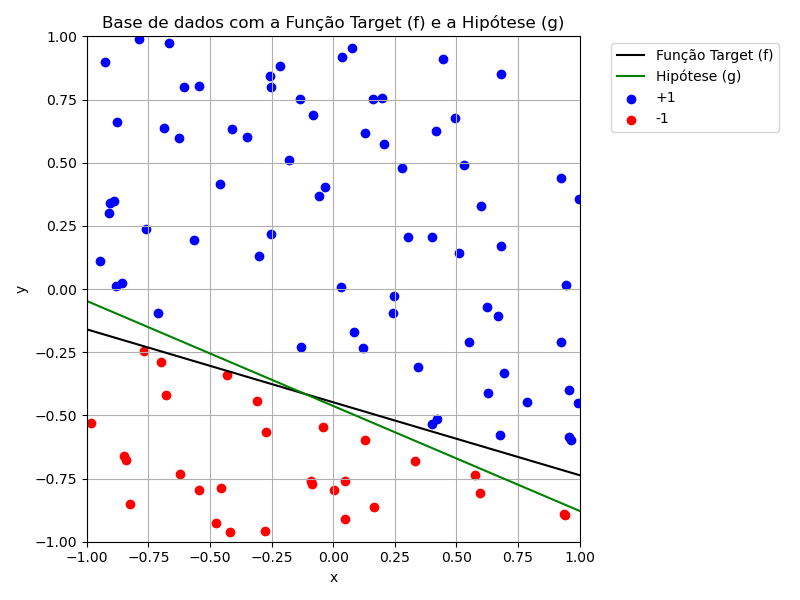
\includegraphics[width=12cm]{perceptron_plot.png}
    \label{fig:perceptron_plot}
\end{figure}

Pela figura \ref{fig:perceptron_plot}, é possível observar que a Hipótese (g) gera uma linha que, apesar de não sobrepor completamente a linha da Função Target (f), separa os pontos perfeitamente, resultado já esperado pelo treinamento utilizando o PLA, uma vez que esse algoritmo só converge quando o erro dentro da amosta $E_{in}$ é nulo.  

\begin{enumerate}
    \item Considere $N = 10$. Quantas iterações demora, em média, para que o PLA convirja com $N = 10$
    pontos de treinamento? Escolha o valor mais próximo do seu resultado.

    \begin{enumerate}
        \item[\textcolor{red}{(a)}]\textcolor{red}{1}\addtocounter{enumii}{1}
        \item 15 *
        \item 300
        \item 5000
        \item 10000
    \end{enumerate}
     
    \par

    \textbf{Justificativa:}

    Para responder a esse item foi implementada a seguinte função:

    \begin{lstlisting}[language=Python, caption=Cálculo do número de iterações, label=cod:perceptron_num_iter]
        def calc_num_iter(num_points, verbose = True):
        lista_iter = list()
        for _ in range(1000):
            target = Target()
            target.generate_random_line()
            dataset = Dataset(num_points)
            data, labels = dataset.generate_dataset(target)
            perceptron = Perceptron2D()
            iter, _ = perceptron.pla(data,labels)
            lista_iter.append(iter)
        if verbose: print(f"{np.mean(lista_iter)} iterações com desvio padrão {np.std(lista_iter):.4f} (min:{np.min(lista_iter)}, máx:{np.max(lista_iter)})")
        return lista_iter
    \end{lstlisting}

    O resultado após 1000 execuções do experimento, com a variável $num\_points = 10$, foi uma média de $5.0490(\approx 5)$ iterações, com desvio padrão de $7.7770(\approx 8)$ iterações, mínimo de 2 iterações e máximo de 99 iterações. Nota-se que o número de iterações pode variar bastante entre uma execução e outra, o que se deve ao alto grau de aleatoriedade presente no problema, uma vez que tanto os pontos quanto a reta da Função Target são gerados de forma aleatória, podendo levar a configurações de diferentes níveis de dificuldade para o PLA convergir. 
    % Apesar de toda essa aleatoriedade, em todas as execuções da função $calc\_num\_iter(num\_points)$ a média se manteve em torno de 5, tendo variando apenas o devio padrão.
     Como 5 está mais próximo de 1 do que de 15, o \textcolor{red}{\textbf{item a}} foi selecionado. 
    
    \item Qual das alternativas seguintes é mais próxima de $\mathbb{P}[f(x) \neq g(x)]$ para $N = 10$?
    
    \begin{enumerate}
        \item 0.001
        \item 0.01
        \item[\textcolor{red}{(c)}]\textcolor{red}{0.1}\addtocounter{enumii}{1}
        \item 0.5
        \item 1
    \end{enumerate}
     
    \par

    \textbf{Justificativa:}
     
    $\mathbb{P}[f(x) \neq g(x)]$ pode ser estimada computacionalmente gerando-se uma quiantidade suficientemente grande de pontos novos e calculando o percentual de erro na classificação desses pontos. Para responder esse item foram realizadas 1000 execuções, nas quais foram gerados 10010 pontos, sendo 10 utilizados para o treinamento do perceptron e 10 mil utilizados para teste. A cada execução foi calculado o perceltual de erro, isto é, a quantidade de vezes que a classificação do perceptron foi diferente da função target divido pela quantidade de pontos. No final das execuções, $\mathbb{P}[f(x) \neq g(x)]$ foi estimada fazendo a média do percentual de erro em cada execução. A Implementação pode ser vista abaixo:

    \begin{lstlisting}[language=Python, caption=Cálculo da probabilidade de erro, label=cod:perceptron_p_erro]
        def calc_p_erro(num_points, verbose = True):
        lista_erro = list()
        for _ in range(1000):
            target = Target()
            target.generate_random_line()
            dataset_train = Dataset(num_points)
            x_train, y_train = dataset_train.generate_dataset(target)
            dataset_test = Dataset(10000) # mais 10mil pontos
            x_test, y_test = dataset_test.generate_dataset(target)
            perceptron = Perceptron2D()
            perceptron.pla(x_train,y_train)
            y_predicted = perceptron.classificar(x_test)
            erro = np.mean(y_test != y_predicted)
            lista_erro.append(erro)
        if verbose: print(f"P[f(x)\u2260g(x)] = {np.mean(lista_erro):.4f}")
        return lista_erro
    \end{lstlisting}

    O resultado após 1000 execuções, com $num\_points = 10010$ e $train\_size = 10$, foi  $\mathbb{P}[f(x) \neq g(x)] = 0.0671 = 6.71\%$. Como 0.0671 está mais próximo de 0.1 do que de 0.01, o \textcolor{red}{\textbf{item c}} foi selecionado. 

    \item Agora considere $N = 100$. Quantas iterações demora, em média, para que o PLA convirja com
    N = 100 pontos de treinamento? Escolha o valor mais próximo do seu resultado.

    \begin{enumerate}
        \item[\textcolor{red}{(a)}]\textcolor{red}{50}\addtocounter{enumii}{1}
        \item 100 *
        \item 500 
        \item 1000
        \item 5000
    \end{enumerate}
     
    \par

    \textbf{Justificativa:}

    Para responder a este item foi utilizada a mesma função do item 1 (código \ref{cod:perceptron_num_iter}), com $num\_points = 100$. 
    
    O resultado após 1000 execuções do experimento foi uma média de $32.981 (\approx 33)$ iterações, com desvio padrão de $164.5924 (\approx 165)$ iterações, mínimo de 2 iterações e máximo de 49 iterações. Nota-se que novamente o número de iterações pode variar bastante entre uma execução e outra, conforme já observado e explicado no item 1. Como 33 está abaixo de 50 e não existe alternativa menor, o \textcolor{red}{\textbf{item a}} foi selecionado. 
     

    \item Qual das alternativas seguintes é mais próxima de $\mathbb{P}[f(x) \neq g(x)]$ para $N = 100$?
    
    \begin{enumerate}
        \item 0.001
        \item[\textcolor{red}{(b)}]\textcolor{red}{0.01}\addtocounter{enumii}{1}
        \item 0.1
        \item 0.5
        \item 1
    \end{enumerate}

    \par

    \textbf{Justificativa:}

    Para responder a este item foi utilizada a mesma função do item 2 (código \ref{cod:perceptron_p_erro}), com $num\_points = 100$.

    O resultado após 1000 execuções foi  $\mathbb{P}[f(x) \neq g(x)] = 0.0069 = 0.69\%$. Como 0.0069 está mais próximo de 0.01 do que de 0.001, o \textcolor{red}{\textbf{item b}} foi selecionado. 
     
    
    \item  É possível estabelecer alguma regra para a relação entre $N$, o número de iterações até a convergência,
    e $\mathbb{P}[f(x) \neq g(x)]$?

    \par

    \textbf{Resposta:}

    Para responder a este item foram implementadas duas funções: uma para calcular o número de iterações e $\mathbb{P}[f(x) \neq g(x)]$ para uma faixa de diferentes números de pontos (código \ref{cod:perceptron_relationship}) e outra para plotar os resultados (código \ref{cod:perceptron_relationship_plot}). O código das duas pode ser observado abaixo.


    \begin{lstlisting}[language=Python, caption=Cálculo da probabilidade de erro e do número de iterações, label=cod:perceptron_relationship]
        def relationship(lista_num_points):
            lista_iter_medio = list()
            lista_erro_medio = list()
            for num_points in lista_num_points:
                lista_iter = calc_num_iter(num_points, verbose=False)
                lista_erro = calc_p_erro(num_points, verbose=False)
                lista_iter_medio.append(np.mean(lista_iter))  
                lista_erro_medio.append(np.mean(lista_erro))
            return lista_iter_medio, lista_erro_medio
    \end{lstlisting}

    \begin{lstlisting}[language=Python, caption=Plot da probabilidade de erro e do número de iterações, label=cod:perceptron_relationship_plot]
        def plot_relationship(num_points_list, lista_iter_medio, lista_erro_medio):
            fig, ax = plt.subplots(1, 1, figsize=(8, 8))
            ax.plot(num_points_list,lista_iter_medio,c="blue",label="Iterações")
            ax.set_title("Curvas de relação")
            ax.set_xlabel('Nº de pontos')
            ax.set_ylabel('Iterações')
            ax2=ax.twinx()
            ax2.plot(num_points_list,lista_erro_medio,c="red", label='P[f(x)\u2260g(x)]')
            ax2.set_ylabel('P[f(x)\u2260g(x)]')
            fig.legend(loc='upper center', bbox_to_anchor=(0.5, 0.9))
            fig.tight_layout()
            plt.show()
    \end{lstlisting}

    O resultado para o tamanho $N$ da amostra variando de 10 a 100 com passo 2 pode ser observado na figura \ref{fig:perceptron_relationship_plot}. 

    \begin{figure}[H]
        \caption{Resultado para $N$ variando de 10 a 100 com passo 2}
           \centering
           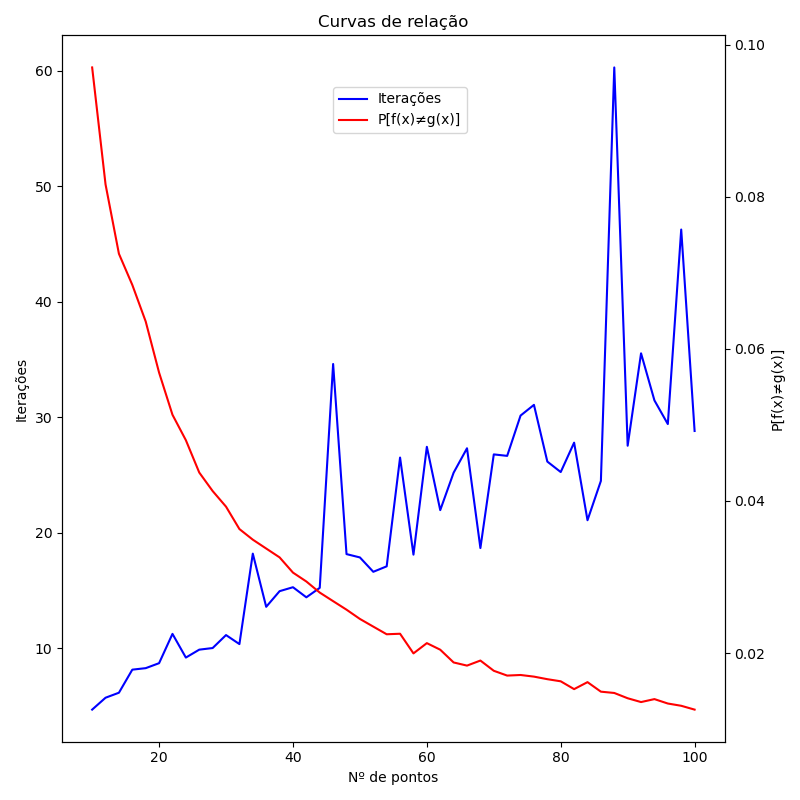
\includegraphics[width=12cm]{perceptron_relationship_plot.png}
        \label{fig:perceptron_relationship_plot}
    \end{figure}

    A quantidade de iterações para o PLA convergir, como constatado nos itens 1 e 3, oscila bastante, porém, pela figura, é possível observar que ela tem uma tendencia de alta conforme $N$ aumenta. Já a probabilidade de erro $\mathbb{P}[f(x) \neq g(x)]$ visivelmente apresenta uma queda exponencial com o aumento de $N$. Conclui-se que, com o aumento de $N$, o algoritmo se torna mais confiável, porém demora mais para ser treinado.
    
    
\end{enumerate}